\documentclass{article}
\usepackage{graphicx}
\usepackage[spanish]{babel}
\usepackage[utf8]{inputenc}
\usepackage{listings}
\usepackage{caption} 

\captionsetup{skip=-30pt}

\pagenumbering{gobble}


\begin{document}

\title{Sistemas de Gestión de Datos y de la Información. Práctica 2. \\ K\_means.}
\author{Alberto Lorente y Hristo Ivanov}
\maketitle

  \begin{abstract}
     Evaluación de la calidad del \emph{clustering} para valores de k entre 2 y 20.
  \end{abstract}

  \section{Resultados}
    Para empezar hacemos una pequeña aclaración de que las líneas verticales del gráfico
    representan el máximo y mínimo, mientras que la línea azul respresenta la media ponderada.
    \par
    Cuando el valor mínimo para una \texttt{k} es \texttt{0}, es porque algun \emph{cluster}
    tiene un solo elemento, incluso un \emph{cluster} puede llegar a quedarse vacio.    

    \begin{figure}[h]
      \centering
      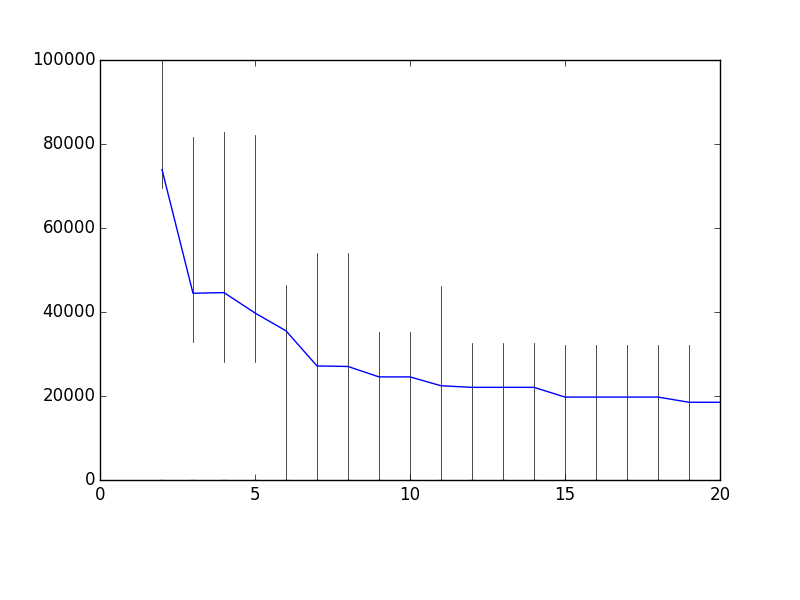
\includegraphics[height=0.4\textheight, width=1\textwidth]{../k-means/Radios.png}
      \caption{Radios}
      \label{fig:radios}
    \end{figure}

    \begin{figure}
      \centering
      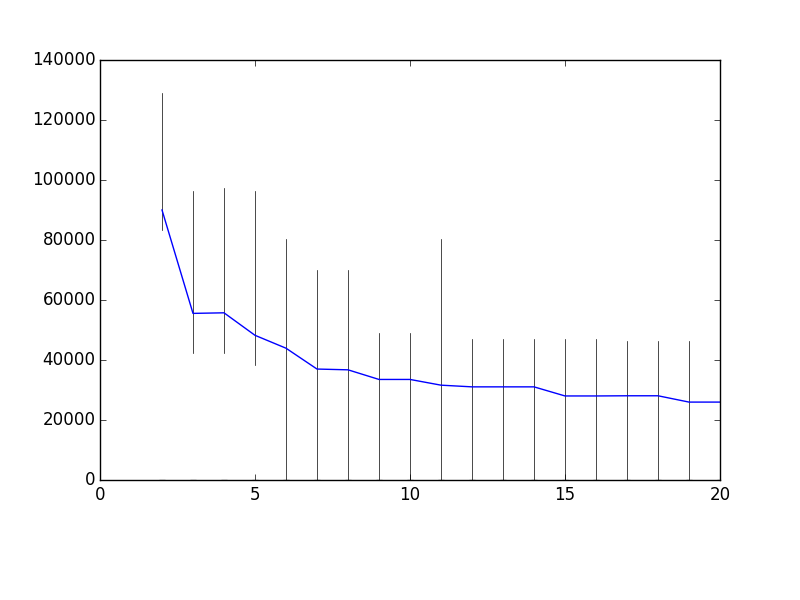
\includegraphics[keepaspectratio, width=1\textwidth]{../k-means/Diametros.png}
      \caption{Diametros}
      \label{fig:diam}
      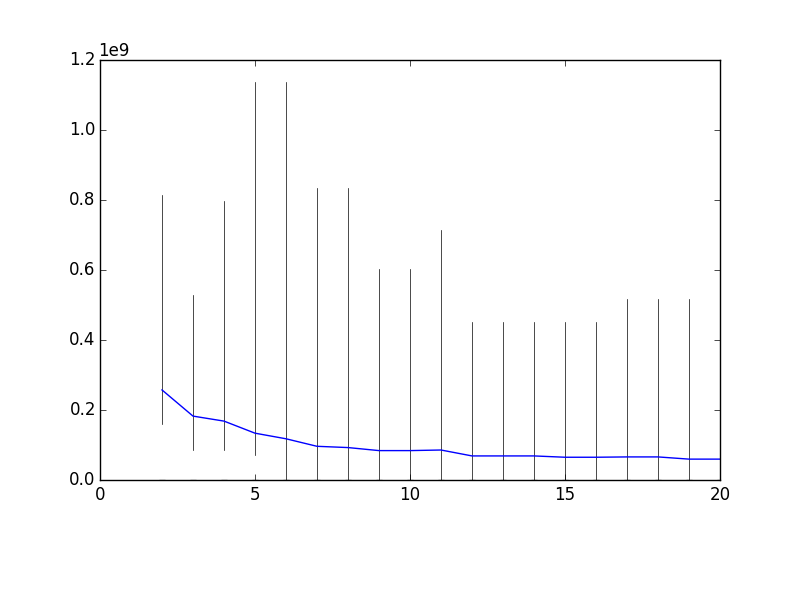
\includegraphics[keepaspectratio, width=1\textwidth]{../k-means/Distancia.png}
      \caption{Distancia}
      \label{fig:dist}
    \end{figure}

  \section{Conclusiones}
    Como podemos ver en las figuras anteriores, cuanto menor es la \texttt{k} 
    peor es la calidad de los \emph{clusters} con respecto a su Radio, Distancia y 
    Diámetro. Segun aumentamos el número de \emph{clusters} podemos observar como
    mejora la calidad de los mismo.
    \par
    No obstante apartir de \texttt{k=7} podemos observar que la ganancia de cohesión
    de los \emph{clusters} no mejora de forma significativa. Además con \texttt{k=7}
    tan solo tenemos un \emph{cluster} con un solo elemento. Para \texttt{k>7} el
    número de \emph{clusters} que tienen un único elemento o ninguno aumenta.  
    \par
    Basandonos en lo anterior concluimos que mejor opción es \texttt{k=7}.  
    


\end{document}
